\documentclass[journal,12pt,twocolumn]{IEEEtran}

\usepackage{setspace}
\usepackage{gensymb}

\singlespacing


\usepackage[cmex10]{amsmath}

\usepackage{amsthm}
\usepackage[utf8]{inputenc}
\usepackage{graphicx}
\usepackage{mathrsfs}
\usepackage{txfonts}
\usepackage{stfloats}
\usepackage{bm}
\usepackage{cite}
\usepackage{cases}
\usepackage{subfig}

\usepackage{longtable}
\usepackage{multirow}

\usepackage{enumitem}
\usepackage{mathtools}
\usepackage{steinmetz}
\usepackage{tikz}
\usepackage{circuitikz}
\usepackage{verbatim}
\usepackage{tfrupee}
\usepackage[breaklinks=true]{hyperref}
\usepackage{graphicx}
\usepackage{tkz-euclide}
\usepackage{epsfig}
\usepackage{}
\usetikzlibrary{calc,math}
\usepackage{listings}
    \usepackage{color}                                            %%
    \usepackage{array}                                            %%
    \usepackage{longtable}                                        %%
    \usepackage{calc}                                             %%
    \usepackage{multirow}                                         %%
    \usepackage{hhline}                                           %%
    \usepackage{ifthen}                                           %%
    \usepackage{lscape}     
\usepackage{multicol}
\usepackage{chngcntr}

\DeclareMathOperator*{\Res}{Res}

\renewcommand\thesection{\arabic{section}}
\renewcommand\thesubsection{\thesection.\arabic{subsection}}
\renewcommand\thesubsubsection{\thesubsection.\arabic{subsubsection}}

\renewcommand\thesectiondis{\arabic{section}}
\renewcommand\thesubsectiondis{\thesectiondis.\arabic{subsection}}
\renewcommand\thesubsubsectiondis{\thesubsectiondis.\arabic{subsubsection}}


\hyphenation{op-tical net-works semi-conduc-tor}
\def\inputGnumericTable{}                                 %%

\lstset{
%language=C,
frame=single, 
breaklines=true,
columns=fullflexible
}
\begin{document}


\newtheorem{theorem}{Theorem}[section]
\newtheorem{problem}{Problem}
\newtheorem{proposition}{Proposition}[section]
\newtheorem{lemma}{Lemma}[section]
\newtheorem{corollary}[theorem]{Corollary}
\newtheorem{example}{Example}[section]
\newtheorem{definition}[problem]{Definition}

\newcommand{\BEQA}{\begin{eqnarray}}
\newcommand{\EEQA}{\end{eqnarray}}
\newcommand{\define}{\stackrel{\triangle}{=}}
\bibliographystyle{IEEEtran}
\providecommand{\mbf}{\mathbf}
\providecommand{\pr}[1]{\ensuremath{\Pr\left(#1\right)}}
\providecommand{\qfunc}[1]{\ensuremath{Q\left(#1\right)}}
\providecommand{\sbrak}[1]{\ensuremath{{}\left[#1\right]}}
\providecommand{\lsbrak}[1]{\ensuremath{{}\left[#1\right.}}
\providecommand{\rsbrak}[1]{\ensuremath{{}\left.#1\right]}}
\providecommand{\brak}[1]{\ensuremath{\left(#1\right)}}
\providecommand{\lbrak}[1]{\ensuremath{\left(#1\right.}}
\providecommand{\rbrak}[1]{\ensuremath{\left.#1\right)}}
\providecommand{\cbrak}[1]{\ensuremath{\left\{#1\right\}}}
\providecommand{\lcbrak}[1]{\ensuremath{\left\{#1\right.}}
\providecommand{\rcbrak}[1]{\ensuremath{\left.#1\right\}}}
\theoremstyle{remark}
\newtheorem{rem}{Remark}
\newcommand{\sgn}{\mathop{\mathrm{sgn}}}
\providecommand{\abs}[1]{\left\vert#1\right\vert}
\providecommand{\res}[1]{\Res\displaylimits_{#1}} 
\providecommand{\norm}[1]{\left\lVert#1\right\rVert}
%\providecommand{\norm}[1]{\lVert#1\rVert}
\providecommand{\mtx}[1]{\mathbf{#1}}
\providecommand{\mean}[1]{E\left[ #1 \right]}
\providecommand{\fourier}{\overset{\mathcal{F}}{ \rightleftharpoons}}
%\providecommand{\hilbert}{\overset{\mathcal{H}}{ \rightleftharpoons}}
\providecommand{\system}{\overset{\mathcal{H}}{ \longleftrightarrow}}
	%\newcommand{\solution}[2]{\textbf{Solution:}{#1}}
\newcommand{\solution}{\noindent \textbf{Solution: }}
\newcommand{\cosec}{\,\text{cosec}\,}
\providecommand{\dec}[2]{\ensuremath{\overset{#1}{\underset{#2}{\gtrless}}}}
\newcommand{\myvec}[1]{\ensuremath{\begin{pmatrix}#1\end{pmatrix}}}
\newcommand{\mydet}[1]{\ensuremath{\begin{vmatrix}#1\end{vmatrix}}}
\numberwithin{equation}{subsection}
\makeatletter
\@addtoreset{figure}{problem}
\makeatother
\let\StandardTheFigure\thefigure
\let\vec\mathbf
\renewcommand{\thefigure}{\theproblem}
\def\putbox#1#2#3{\makebox[0in][l]{\makebox[#1][l]{}\raisebox{\baselineskip}[0in][0in]{\raisebox{#2}[0in][0in]{#3}}}}
     \def\rightbox#1{\makebox[0in][r]{#1}}
     \def\centbox#1{\makebox[0in]{#1}}
     \def\topbox#1{\raisebox{-\baselineskip}[0in][0in]{#1}}
     \def\midbox#1{\raisebox{-0.5\baselineskip}[0in][0in]{#1}}
\vspace{3cm}
\title{Assignment 1}
\maketitle
\newpage
\bigskip
\renewcommand{\thefigure}{\theenumi}
\renewcommand{\thetable}{\theenumi}
Download all python codes from 
\begin{lstlisting}
https://github.com/behappy0604/Assignment1
\end{lstlisting}
%
and latex-tikz codes from 
%
\begin{lstlisting}
https://github.com/behappy0604/Assignment1
\end{lstlisting}
%
\section{constr-2.27 part1}
\ Construct a triangle: $\angle$A = 85 $^{\circ}$ ,$\angle$B = 115 $^{\circ}$ and AB = 5.

\section{Exaplanation}
%
\tikzset{every picture/.style={line width=0.75pt}} %set default line width to 0.75pt        

\begin{tikzpicture}[x=0.75pt,y=0.75pt,yscale=-1,xscale=1]
%uncomment if require: \path (0,300); %set diagram left start at 0, and has height of 300

%Straight Lines [id:da07068098265908507] 
\draw    (304,62) -- (424,182) ;
%Straight Lines [id:da9183397026045734] 
\draw    (304,62) -- (291,180) ;
%Straight Lines [id:da6639889359129583] 
\draw    (291,180) -- (424,182) ;
%Shape: Arc [id:dp23297095368791165] 
\draw  [draw opacity=0] (401.04,179.95) .. controls (401.01,179.47) and (401,178.99) .. (401,178.5) .. controls (401,172.98) and (402.62,167.81) .. (405.44,163.39) -- (432.5,178.5) -- cycle ; \draw   (401.04,179.95) .. controls (401.01,179.47) and (401,178.99) .. (401,178.5) .. controls (401,172.98) and (402.62,167.81) .. (405.44,163.39) ;
%Shape: Arc [id:dp5218605505907268] 
\draw  [draw opacity=0] (315.87,180.32) .. controls (314.82,174.14) and (310.73,168.19) .. (303.36,162.97) .. controls (300.04,160.63) and (296.22,158.54) .. (291.99,156.73) -- (227,190) -- cycle ; \draw   (315.87,180.32) .. controls (314.82,174.14) and (310.73,168.19) .. (303.36,162.97) .. controls (300.04,160.63) and (296.22,158.54) .. (291.99,156.73) ;

% Text Node
\draw (345,188) node [anchor=north west][inner sep=0.75pt]  [font=\scriptsize] [align=left] {5};
% Text Node
\draw (278,178) node [anchor=north west][inner sep=0.75pt]   [align=left] {A};
% Text Node
\draw (434.5,181.5) node [anchor=north west][inner sep=0.75pt]   [align=left] {B};
% Text Node
\draw (296,46) node [anchor=north west][inner sep=0.75pt]   [align=left] {C};
% Text Node
\draw (376,168) node [anchor=north west][inner sep=0.75pt]  [font=\tiny] [align=left] {115$ $};
% Text Node
\draw (313,155) node [anchor=north west][inner sep=0.75pt]  [font=\tiny] [align=left] {85};


\end{tikzpicture}

The above mentioned triangle cannot be formed.
As if we do addition of both angles $\angle$A and $\angle$B

85$^{\degree}$+115$^{\degree}$= 200$^{\degree}$

But according to the theorem sum of all angles of triangle =180$^{\degree}$
so here, $ 200\degree > 180\degree $
Hence triangle cannot be formed.
\begin{figure}[htp]
    \centering
    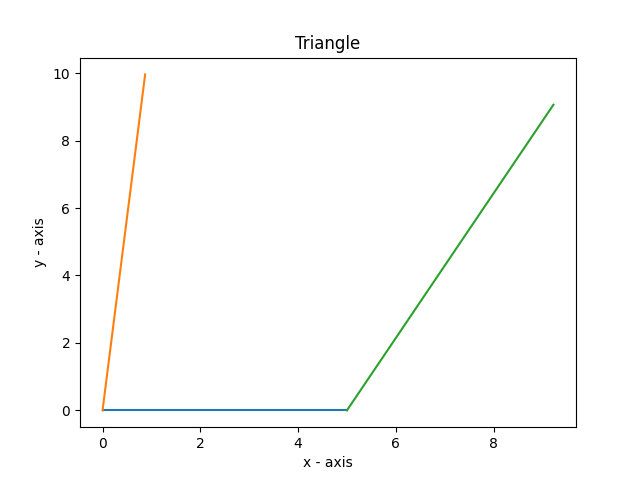
\includegraphics[width=8cm]{Figure_1.png}
    \caption{ Constructed a triangle using python}
\end{figure}
\end{document}
